\documentclass[10pt,letterpaper]{article}
\usepackage[margin=0.65in]{geometry}
\usepackage[T1]{fontenc}
\usepackage{newtxtext,newtxmath}
\usepackage{microtype,multicol,booktabs,graphicx,caption,fancyhdr,array}
\usepackage[table]{xcolor}
\definecolor{teal}{HTML}{006B68}
\definecolor{navy}{HTML}{17384A}
\definecolor{pale}{HTML}{EAF5F3}
\definecolor{slate}{HTML}{EDF1F4}
\renewcommand{\arraystretch}{1.13}
\usepackage[hidelinks]{hyperref}
\setlength{\columnsep}{0.25in}
\setlength{\parindent}{0.8em}
\setlength{\parskip}{2pt}
\captionsetup{font=small,labelfont=bf,skip=4pt,hypcap=false}
\usepackage{titlesec}
\titleformat{\section}{\normalsize\sffamily\bfseries\color{navy}}{\thesection.}{0.4em}{}
\titlespacing*{\section}{0pt}{8pt}{4pt}
\pagestyle{fancy}\fancyhf{}
\fancyhead[L]{\scriptsize MINIMALIST EDGE AI CHALLENGE}
\fancyhead[R]{\scriptsize SOFTWARE OPTIMIZATION TRACK}
\fancyfoot[C]{\small\thepage}
\renewcommand{\headrulewidth}{0.3pt}
\setlength{\headheight}{13pt}
\setlength{\footskip}{20pt}
\newcommand{\code}[1]{\texttt{\small #1}}
\begin{document}
\begin{center}
{\LARGE\bfseries\color{navy} Calibrated INT8 Quantization:\\[3pt] Efficient EuroSAT Inference with Minimal Accuracy Loss}\\[6pt]
{\small Minimalist Edge AI Challenge\quad\textbullet\quad Software Track\quad\textbullet\quad 13 October 2026}
\end{center}
\vspace{-5pt}
\noindent\textbf{Abstract.} We optimize a supplied MobileNetV2 student for satellite land-use classification using static INT8 quantization. Per-channel weights and 99.99th-percentile calibration deliver our best verified accuracy--efficiency balance without retraining. The selected model, Q3a, retains 99.76\% of baseline accuracy and achieves a $4.29\times$ speedup in Qualcomm AI Hub's proxy-device profile. We select it over a smaller pruned model whose accuracy did not recover within the available training budget.

\begin{center}
\setlength{\fboxsep}{8pt}
\colorbox{pale}{\begin{minipage}{0.955\textwidth}
\centering\sffamily
\begin{tabular*}{\linewidth}{@{\extracolsep{\fill}}cccc@{}}
\textbf{\large\color{teal}98.92\%} & \textbf{\large\color{teal}70.7\% smaller} & \textbf{\large\color{teal}3.06$\times$ faster} & \textbf{\large\color{teal}67.7\% less energy}\\
\small Overall accuracy & \small 8.506 $\to$ 2.491 MiB & \small 2.554 $\to$ 0.836 ms & \small CPU estimate per image
\end{tabular*}
\end{minipage}}
\end{center}
\vspace{3pt}
\begin{multicols}{2}
\section{The task and our test setup}
The supplied student classifies EuroSAT RGB imagery into ten land-use classes. We preserve the required FP32 input named \code{input}, shape $(1,3,224,224)$, and ten output scores. Images are resized to $224\times224$, converted to tensors, and normalized with the supplied ImageNet mean and standard deviation.

Following the judge instruction recorded in the project, final accuracy is evaluated on all 27,000 images, including calibration images. Consequently, it is a full-dataset competition measurement, not an independent held-out generalization estimate. All baseline numbers here are our local measurements; organizer-provided \code{baseline\_metrics.json} was unavailable.

We export the unchanged checkpoint with ONNX opset 13 and \code{dynamo=False}, and use ONNX Runtime 1.31.0 with its CPU execution provider. Export-verification code compares real-image logits and predicted classes with PyTorch. Using ONNX for both baseline and final comparisons avoids attributing a runtime change to compression.



Local measurements use an 11-core Apple M3 Pro, 18 GB RAM, mains power, batch one, and ONNX Runtime's default thread setting. The milestone alternates candidates over five rounds; each round uses ten warm-ups, 100 timed inferences, and a 15-second energy run. Table~\ref{tab:final} uses the median across rounds, with median inference latency within each round. RAM is sampled process RSS, not model storage.
\section{How we chose the winning model}
Our pipeline is checkpoint $\rightarrow$ FP32 ONNX $\rightarrow$ graph preprocessing $\rightarrow$ calibration $\rightarrow$ static INT8 QDQ $\rightarrow$ validation. Preprocessing performs shape inference and graph optimization before quantization. QDQ represents quantization explicitly with QuantizeLinear and DequantizeLinear nodes; static ranges are calibrated before deployment~\cite{ort}.

The principal calibration set contains 300 fixed images, 30 per class, sampled with seed 42. We compare per-tensor and per-channel weight scales, signed/unsigned activation types, MinMax, entropy and percentile calibration, and selective FP32 retention. The selected Q3a configuration uses signed INT8 weights and activations (S8S8), per-channel weights, 99.99th-percentile calibration, and no excluded layers. No retraining is needed for this selected artifact.

\begin{center}
\captionof{table}{Quantization study on all 27,000 images. Size uses $2^{20}$ bytes (MiB).}
\label{tab:ablation}
\small\setlength{\tabcolsep}{3pt}
\begin{tabular}{@{}lrr@{}}
\toprule
\rowcolor{slate}\textbf{Configuration} & \textbf{Acc. (\%)} & \textbf{MiB}\\
\midrule
Original FP32 & 99.16 & 8.506\\
Q0: per-tensor, MinMax, U8S8 & 96.32 & 2.277\\
Q1: per-channel, MinMax, S8S8 & 98.09 & 2.491\\
Q1b: Q1 with U8S8 & 98.09 & 2.491\\
Q2: per-channel, entropy & 98.09 & 2.491\\
\rowcolor{pale}\textbf{Q3a: percentile 99.99} & \textbf{98.92} & \textbf{2.491}\\
Q3b: percentile 99.999 & 98.69 & 2.491\\
Q4: Q3a, first/last layers FP32 & 98.86 & 2.528\\
Q6: 100 / 1,000 calibration images & 98.83 / 98.90 & 2.491\\
Q7: FP16 & 99.17 & 4.285\\
\bottomrule
\end{tabular}
\end{center}

\noindent\textbf{Selection rationale.} Q1b versus Q0 isolates weight-scale granularity at U8S8 and improves accuracy by 1.77 percentage points. Q3a then gains 0.83 points over per-channel MinMax. Increasing the percentile to 99.999 retains more extreme values but performs worse here. Protecting the first and last layers also fails to improve accuracy. The 100- and 1,000-image checks remain within 0.09 points of the 300-image result; this supports that choice in this experiment, without establishing general convergence.

Q3a meets our targets of at least 98.9\% overall accuracy, about 95\% on PermanentCrop, and at most 2.5 MiB. FP16 preserves accuracy but is larger and slightly slower than FP32 in our repeated CPU benchmark (2.708 versus 2.554 ms). Cross-layer equalization~\cite{dfq}, adaptive rounding and quantization-aware training were considered but are not claimed as completed experiments.
\end{multicols}
\newpage
\begin{center}
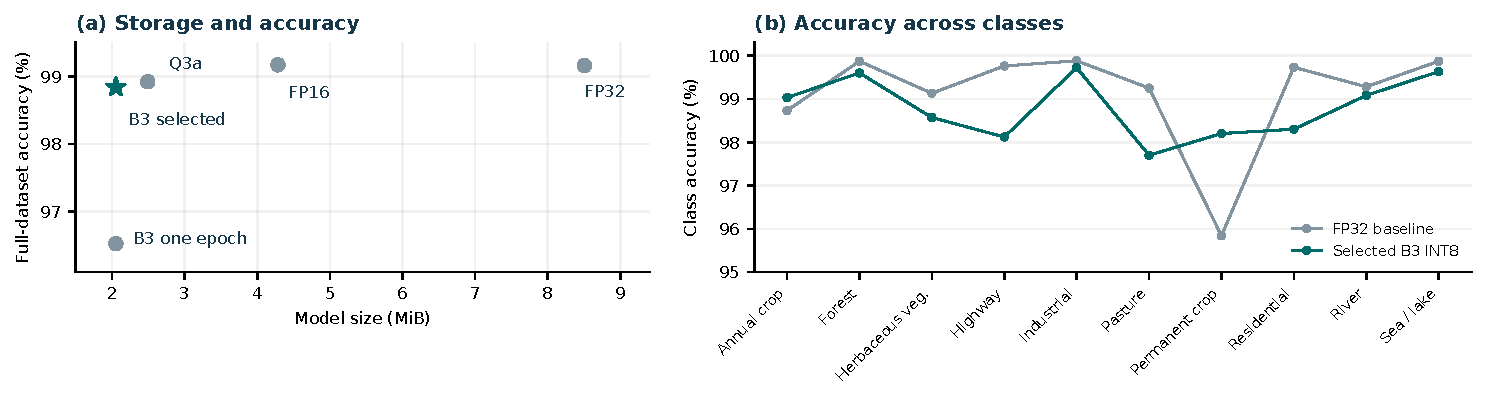
\includegraphics[width=\textwidth]{tradeoff.pdf}
\vspace{-9pt}
\captionof{figure}{Quantization tradeoffs on all 27,000 EuroSAT images. (a) Accuracy versus storage for representative candidates; the line joins selected tradeoff points. (b) The three finalists measured in the same five-round local benchmark. Q3a is highlighted: 98.92\% accuracy at 2.491 MiB and 0.836 ms per image.}
\end{center}
\vspace{-7pt}
\begin{multicols}{2}
\section{What the winning model achieved}
\begin{center}
\begin{minipage}{\linewidth}
\centering
\captionof{table}{Selected model versus identical-runtime baseline.}
\label{tab:final}
\small\setlength{\tabcolsep}{4pt}
\begin{tabular}{@{}lrr@{}}
\toprule
\rowcolor{slate}\textbf{Metric} & \textbf{FP32} & \textbf{Q3a INT8}\\
\midrule
\rowcolor{pale}Overall accuracy (\%) & 99.16 & 98.92\\
Worst class: PermanentCrop (\%) & 95.84 & 95.24\\
\rowcolor{pale}File size (MiB) & 8.506 & 2.491\\
Parameters (M) / MACs (G) & 2.220 / 0.2995 & same\\
\rowcolor{pale}Local median latency (ms) & 2.554 & 0.836\\
Local peak RSS (MiB) & 87.91 & 76.86\\
\rowcolor{pale}Estimated energy (J/image) & 0.05993 & 0.01938\\
AI Hub estimated latency (ms) & 26.690 & 6.225\\
AI Hub estimated peak (MiB) & 28.10 & 29.35\\
\bottomrule
\end{tabular}
\end{minipage}
\end{center}

Q3a reduces storage by 70.7\% ($3.41\times$ smaller) and median local latency by 67.3\% ($3.06\times$ faster), while losing only 0.24 percentage points of accuracy. It retains 99.76\% of baseline accuracy; no class loses more than 0.95 points. Local peak RSS falls 12.6\%. Parameters and MACs remain unchanged: these gains come from lower-precision representation and execution, not structural removal. Estimated energy falls 67.7\%; CodeCarbon uses a CPU-load/TDP estimate rather than power sensors, with variation across rounds.

\noindent\textbf{Device choice.} We used the Dragonwing RB3 Gen 2 Vision Kit (QCS6490, Qualcomm Linux 1.6). The project catalog check found no UNO Q / QRB2210 profile and selected this lower-tier listed Linux IoT alternative. Both saved ONNX profiles execute entirely on CPU. AI Hub estimates a $4.29\times$ speedup, while peak memory rises 4.5\%. These are proxy-device results, not UNO Q measurements or evidence of NPU acceleration.

\section{Pruning + INT8: lessons for next time}
We removed blocks 6, 9 and 16, trained for one epoch with teacher distillation on 5,400 images, and recalibrated INT8. The extra compression cost too much accuracy:
\begin{center}
\begin{minipage}{\linewidth}
\centering\small\setlength{\tabcolsep}{4pt}
\begin{tabular}{@{}lrr@{}}
\toprule
\rowcolor{slate}\textbf{Comparison} & \textbf{Q3a (chosen)} & \textbf{Pruned + INT8}\\
\midrule
Accuracy (\%) & 98.92 & 96.52\\
PermanentCrop (\%) & 95.24 & 89.28\\
Model size (MiB) & 2.491 & 2.052\\
\bottomrule
\end{tabular}
\end{minipage}
\end{center}
\noindent\textbf{What went wrong.} One recovery epoch did not repair the pruning damage: on the same 2,700-image subset, accuracy fell from 97.56\% after pruning/BN adjustment to 96.00\% after training. Full-dataset accuracy was 96.49\% before INT8 and 96.52\% after it, placing the observed deficit before quantization. One epoch consumed 850 seconds (14.2 minutes). We lacked time to tune the learning rate, compare teacher-assisted versus label-only recovery, or complete the separate evaluation excluding fine-tuning images. These results do not establish whether longer recovery would succeed.

\noindent\textbf{Next steps.} Start with fewer removed blocks or milder channel cuts; compare lower learning rates and longer recovery schedules, saving the best validation checkpoint. Test distillation against label-only training, then recalibrate and quantize only recovered candidates. Reserve time for disjoint evaluation and repeated latency/energy measurements. Q3a remains the verified reference to beat.

\section{Reproducibility and conclusion}
The selected \code{student\_model\_int8.onnx} matches Q3a's SHA-256 (prefix \code{3335203487330816}). Rebuild from the supplied checkpoint with \code{export\_onnx.py}, then \code{quantize.py} using \code{--per-channel}, \code{--calib-method percentile}, \code{--percentile 99.99}, and \code{--types s8s8}. Fixed calibration indices and saved settings identify the exact inputs. Use \code{check\_quant.py}, \code{measure.py}, and \code{timing.py} for validation; pruning configurations are saved separately. AI Hub profile IDs are \code{jgk68x4n5} (FP32) and \code{j5wy46y4g} (INT8). For this task and budget, per-channel percentile-calibrated INT8 provides our best verified balance of accuracy, storage and deployment efficiency. The more aggressive pruning extension is retained as evidence for future recovery experiments, rather than selected for submission.

\vspace{-3pt}
\begin{thebibliography}{2}\small
\setlength{\itemsep}{1pt}\setlength{\parskip}{0pt}
\bibitem{ort} ONNX Runtime. \href{https://onnxruntime.ai/docs/performance/model-optimizations/quantization.html}{\emph{Quantize ONNX models}}. Documentation, accessed October 2026.
\bibitem{dfq} M. Nagel et al. \href{https://openaccess.thecvf.com/content_ICCV_2019/html/Nagel_Data-Free_Quantization_Through_Weight_Equalization_and_Bias_Correction_ICCV_2019_paper.html}{Data-Free Quantization Through Weight Equalization and Bias Correction}. \emph{ICCV}, 2019, pp. 1325--1334.
\end{thebibliography}
\end{multicols}
\clearpage
\section*{Appendix A. Dashboard data at a glance}
\noindent\small Recorded experiments from 13 October 2026. Values below come directly from the JSON files behind the dashboard; archived and smoke-test runs are excluded. Teal highlights the submitted model. The first two pages remain the main technical report.
\vspace{5pt}

\noindent\textbf{A1. Full-dataset experiments: all 27,000 EuroSAT images}
\begin{center}
\fontsize{8.5}{10}\selectfont
\setlength{\tabcolsep}{4.3pt}\renewcommand{\arraystretch}{1.2}
\begin{tabular*}{\textwidth}{@{\extracolsep{\fill}}lrrrrrrrrc@{}}
\toprule
\rowcolor{slate}\textbf{Run} & \textbf{Acc.} & \textbf{Worst} & \textbf{Params} & \textbf{MACs} & \textbf{Size} & \textbf{Latency} & \textbf{RAM} & \textbf{Energy} & \textbf{Time}\\
\rowcolor{slate} & \textbf{\%} & \textbf{\%} & \textbf{M} & \textbf{G} & \textbf{MiB} & \textbf{ms} & \textbf{MiB} & \textbf{J/image} & \textbf{basis}\\
\midrule
FP32 ONNX & 99.16 & 95.84 & 2.220 & 0.2995 & 8.506 & 2.554 & 87.91 & 0.05993 & M\\
FP32 PyTorch & 99.16 & 95.84 & 2.237 & 0.3262 & 8.772 & 19.862 & 303.19 & 0.32409 & S\\
Q0 & 96.32 & 88.13 & 2.220 & 0.2995 & 2.277 & 0.905 & 75.56 & 0.02251 & P\\
Q1 & 98.09 & 95.45 & 2.220 & 0.2995 & 2.491 & 0.824 & 76.42 & 0.01843 & P\\
Q1b & 98.09 & 95.45 & 2.220 & 0.2995 & 2.491 & 0.928 & 76.42 & 0.05401 & P\\
Q2 & 98.09 & 95.45 & 2.220 & 0.2995 & 2.491 & 0.835 & 77.17 & 0.02076 & P\\
Q3a: quant-only & 98.92 & 95.24 & 2.220 & 0.2995 & 2.491 & 0.836 & 76.86 & 0.01938 & M\\
Q3b & 98.69 & 95.92 & 2.220 & 0.2995 & 2.491 & 0.836 & 77.08 & 0.01809 & P\\
Q4 & 98.86 & 94.88 & 2.220 & 0.2995 & 2.528 & 1.056 & 77.84 & 0.02448 & P\\
Q6a: 100 images & 98.83 & 94.72 & 2.220 & 0.2995 & 2.491 & 0.912 & 77.16 & 0.11928 & P\\
Q6b: 1,000 images & 98.90 & 94.96 & 2.220 & 0.2995 & 2.491 & 0.838 & 78.52 & 0.03317 & P\\
Q7: FP16 & 99.17 & 95.88 & 2.220 & 0.2995 & 4.285 & 2.708 & 89.33 & 0.06280 & M\\
B3: 1-epoch FP32 & 96.49 & 88.52 & 1.834 & 0.2627 & 7.028 & 2.263 & 83.25 & 0.06386 & P\\
B3: 1-epoch INT8 & 96.52 & 89.28 & 1.834 & 0.2627 & 2.052 & 0.740 & 75.22 & 0.01599 & P\\
B3: 3-epoch FP32 & 98.84 & 97.60 & 1.834 & 0.2627 & 7.028 & 2.302 & 84.27 & 0.06285 & P\\
\rowcolor{pale}\textbf{B3: 3-epoch INT8 (selected)} & \textbf{98.84} & \textbf{97.70} & \textbf{1.834} & \textbf{0.2627} & \textbf{2.052} & \textbf{1.110} & \textbf{77.11} & \textbf{0.04989} & \textbf{P}\\
\bottomrule
\end{tabular*}
\end{center}
\vspace{-4pt}
\noindent\footnotesize\textbf{Reading the table.} M = median of five milestone rounds; P = provisional single-session measurement; S = single-session reference. Latency is the median within a round. All energy values are CodeCarbon estimates; unusually high provisional values should not be treated as settled comparisons. Worst class is Forest for Q0, Pasture for Q1/Q1b/Q2 and the three-epoch B3 runs, and PermanentCrop otherwise. ONNX and PyTorch counts/runtime overhead differ; compare within the same runtime. Q0--Q7 are quantization-only variants. B3 removes blocks 6, 9 and 16; the selected run uses three recovery epochs at learning rate 0.001. Its local timing remains provisional.
\vspace{8pt}

\noindent\small\textbf{A2. Pruning exploration: 2,700-image quick evaluation, before recovery training}

\noindent\footnotesize All candidates use adaptive BN before evaluation. Counts are measured with the same PyTorch/thop method as the reference. These subset accuracies are not directly comparable with A1; latency, RAM and energy were not measured for these Stage A runs.
\vspace{4pt}

\noindent\begin{minipage}[t]{0.49\textwidth}\vspace{0pt}\centering\fontsize{8.5}{10}\selectfont\setlength{\tabcolsep}{2.3pt}\renewcommand{\arraystretch}{1.16}
\begin{tabular*}{\linewidth}{@{\extracolsep{\fill}}lrrrrr@{}}\toprule
\rowcolor{slate}\textbf{Candidate} & \textbf{Acc. \%} & \textbf{Worst \%} & \textbf{Params M} & \textbf{MACs G} & \textbf{MiB}\\\midrule
Reference + BN & 99.37 & 97.60 & 2.237 & 0.3262 & 8.506\\
Drop block 3 & 97.33 & 91.20 & 2.228 & 0.2966 & 8.472\\
Drop block 5 & 98.52 & 93.60 & 2.222 & 0.3139 & 8.449\\
Drop block 6 & 98.96 & 95.60 & 2.222 & 0.3139 & 8.449\\
Drop block 8 & 98.67 & 96.00 & 2.182 & 0.3153 & 8.300\\
Drop block 9 & 98.96 & 95.20 & 2.182 & 0.3153 & 8.300\\
Drop block 10 & 98.48 & 93.20 & 2.182 & 0.3153 & 8.300\\
Drop block 12 & 98.48 & 93.20 & 2.118 & 0.3025 & 8.058\\
Drop block 13 & 98.41 & 95.60 & 2.118 & 0.3025 & 8.058\\
Drop block 15 & 98.44 & 94.00 & 1.917 & 0.3103 & 7.291\\
Drop block 16 & 98.93 & 96.00 & 1.917 & 0.3103 & 7.291\\
Stack 1 block & 98.96 & 95.60 & 2.222 & 0.3139 & 8.449\\
Stack 2 blocks & 98.52 & 93.20 & 2.168 & 0.3030 & 8.243\\
Stack 3 blocks & 97.56 & 92.00 & 1.848 & 0.2871 & 7.028\\
Stack 4 blocks & 94.07 & 84.40 & 1.793 & 0.2761 & 6.822\\
Stack 5 blocks & 91.07 & 79.60 & 1.778 & 0.2638 & 6.764\\
\bottomrule\end{tabular*}
\end{minipage}\hfill
\noindent\begin{minipage}[t]{0.49\textwidth}\vspace{0pt}\centering\fontsize{8.5}{10}\selectfont\setlength{\tabcolsep}{2.3pt}\renewcommand{\arraystretch}{1.16}
\begin{tabular*}{\linewidth}{@{\extracolsep{\fill}}lrrrrr@{}}\toprule
\rowcolor{slate}\textbf{Candidate} & \textbf{Acc. \%} & \textbf{Worst \%} & \textbf{Params M} & \textbf{MACs G} & \textbf{MiB}\\\midrule
Global 10\% & 77.19 & 47.20 & 1.808 & 0.2247 & 6.878\\
Global 20\% & 57.19 & 16.67 & 1.439 & 0.1789 & 5.476\\
Global 30\% & 39.41 & 5.67 & 1.095 & 0.1421 & 4.170\\
Global 40\% & 18.85 & 0.00 & 0.828 & 0.1099 & 3.157\\
Uniform 10\% & 76.26 & 43.20 & 1.784 & 0.2366 & 6.788\\
Uniform 20\% & 65.00 & 51.20 & 1.421 & 0.1984 & 5.409\\
Uniform 30\% & 39.15 & 27.00 & 1.092 & 0.1527 & 4.158\\
Uniform 40\% & 21.37 & 0.00 & 0.810 & 0.1144 & 3.089\\
30\% BN-scale & 15.81 & 0.00 & 1.025 & 0.1584 & 3.903\\
30\% Taylor & 22.74 & 0.00 & 1.003 & 0.1556 & 3.819\\
\bottomrule\end{tabular*}
\par\vspace{8pt}\raggedright\footnotesize
\textbf{Depth-stack key.} Blocks are added in this order: 6, 9, 16, 8, 5. Thus ``Stack 3'' removes 6+9+16; ``Stack 4'' also removes block 8.

\vspace{5pt}\textbf{Width settings.} Global and uniform sweeps use magnitude importance. The requested percentage is a channel-pruning setting, not a percentage of total weights. BN-scale and Taylor are alternative importance criteria at 30\%.

\vspace{5pt}\textbf{Why B3 was selected.} Three-epoch recovery raises INT8 accuracy to 98.84\%. It is 17.6\% smaller than Q3a for a 0.08-point overall-accuracy tradeoff, with a 97.70\% worst-class score. The one-epoch attempt is retained as historical evidence.
\end{minipage}
\par\vspace{8pt}
\noindent\footnotesize\textbf{Source and precision.} A1 uses \code{results/*.json}, replacing timing fields with \code{milestone\_timing} when present, as the dashboard does. A2 uses \code{results/stageA/*.json}. Figures are rounded only for display; the saved JSON records retain the measurement precision. M = million parameters; G = billion multiply--accumulate operations; MiB = $2^{20}$ bytes.


\end{document}
